\documentclass{beamer}

\usepackage{ifpdf}
\ifpdf
\usepackage{hyperref}
%\pdfadjustspacing=1
%\fi

\mode<presentation>
 {
  \usetheme{Frankfurt}
   \usecolortheme[rgb={0.36,0.54,0.66}]{structure}
   
   \definecolor{inaf}{HTML}{1D71B8}
   %\definecolor{ashgrey}{rgb}{0.7, 0.75, 0.71}
   \definecolor{autumn}{rgb}{0.7, 0.75, 0.71}
   \definecolor{autumn1}{rgb}{0.7, 0.75, 0.71}
   \definecolor{autumn2}{rgb}{0.36, 0.54, 0.66}

\setbeamercolor{alerted text}{fg=inaf!80!yellow}
\setbeamercolor*{palette primary}{fg=inaf!60!black,bg=autumn}
\setbeamercolor*{palette secondary}{fg=white!70!black,bg=autumn2}
\setbeamercolor*{palette tertiary}{bg=white!80!black,fg=autumn2}
\setbeamercolor*{palette quaternary}{fg=white,bg=autumn2}

\setbeamercolor*{sidebar}{fg=inaf,bg=autumn}

\setbeamercolor*{palette sidebar primary}{fg=inaf!10!black}
\setbeamercolor*{palette sidebar secondary}{fg=white}
\setbeamercolor*{palette sidebar tertiary}{fg=inaf!50!black}
\setbeamercolor*{palette sidebar quaternary}{fg=yellow!10!orange}

\setbeamercolor*{titlelike}{parent=palette primary}
\setbeamercolor{frametitle}{bg=autumn1}
\setbeamercolor{frametitle right}{bg=autumn}

\setbeamercolor*{separation line}{}
\setbeamercolor*{fine separation line}{}

\mode
<all>
   
   %\usecolortheme{wolverine}
   \usecolortheme{rose}
   \usefonttheme{serif}
%   \setbeamercolor{section in toc}{fg=red}
 }

\title[Universo ottico]{L'universo ottico}
\author[G.Filippelli]{Gianluigi Filippelli}
\date{Liceo "C. Cavalleri", Parabiago (Milano). 23/11/2017}

\usepackage[latin1]{inputenc}
\usepackage[italian]{babel}
\usepackage{times}
%
\begin{document}
%
\begin{frame}
 \titlepage
\end{frame}
%
% Spettro elettromagnetico
%
\section{Lo spettro elettromagnetico}
\begin{frame}[spettro]
	\frametitle{Lo spettro visibile vs tutto il resto!}
	\only<1>{
	\begin{center}
		\href{https://it.wikibooks.org/wiki/Fisica_classica/Spettro_delle_onde_elettromagnetiche}{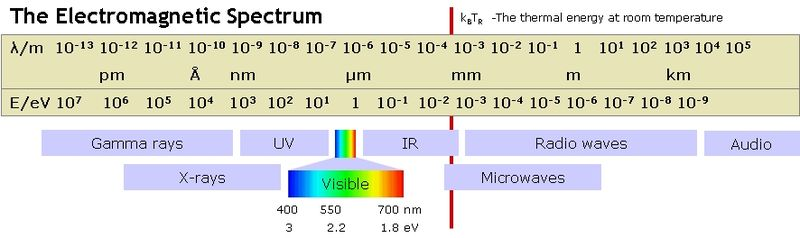
\includegraphics[width=10cm]{files/TheElectromagneticSpectrum.jpg}}
	\end{center}}
	\only<2>{
		\begin{center}
			\href{https://it.wikipedia.org/wiki/Spettro_elettromagnetico}{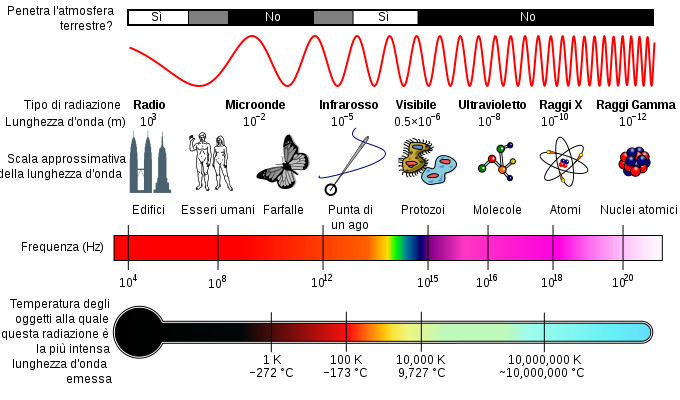
\includegraphics[width=10cm]{files/spettro_elettromagnetico.jpg}}
		\end{center}}
\end{frame}
%
\begin{frame}[onde]
	\frametitle{Le lunghezze d'onda}
	\begin{block}{Osservare il cielo a differenti lunghezze d'onda}
		Le immagini radio evidenziano la presenza di nubi di gas fredde (in particolare l'idrogeno), le immagini in infrarosso mostrano aree a bassa energia, la luce visibile mostra soprattutto gas e polveri, i raggi-x rivelano emissioni ad alta energia.
	\end{block}
\end{frame}
%
% La nebulosa del granchio
%
\section{La nebulosa del granchio}
\subsection{Radio}
\begin{frame}[radio]
	\frametitle{Immagine in radio}
	\begin{center}
		{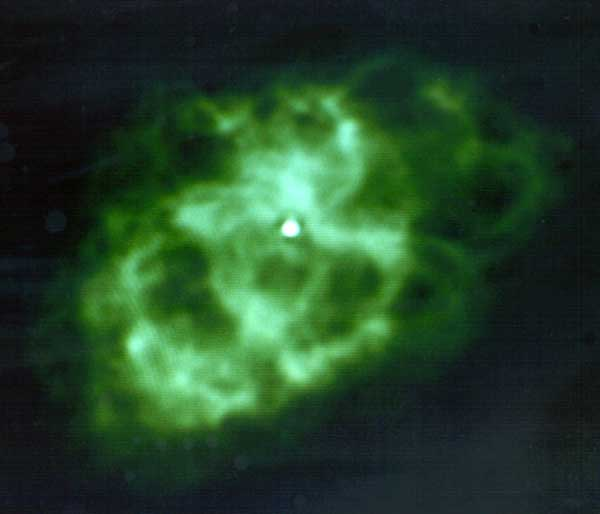
\includegraphics[width=6cm]{files/crab_radio_full.jpg}}
	\end{center}
\end{frame}
%
\subsection{Infrarossi}
%
\begin{frame}[Infrarossi]
	\frametitle{Negli infrarossi}
	\begin{center}
		{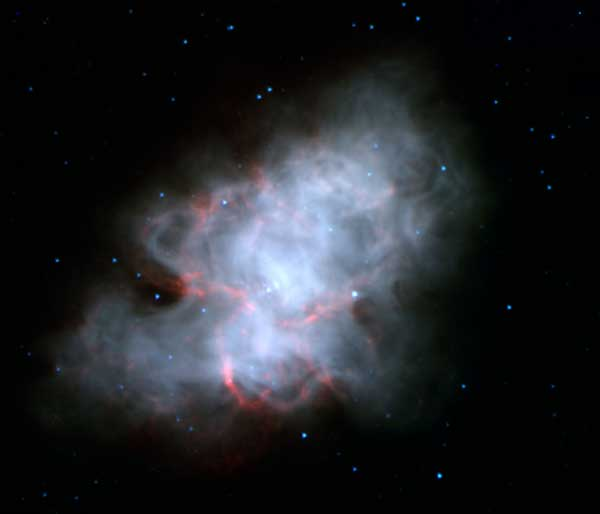
\includegraphics[width=6cm]{files/crab_ir_full.jpg}}
	\end{center}
\end{frame}
%
\subsection{Ottico}
\begin{frame}[ottico]
	\frametitle{Nell'ottico}
	\begin{center}
		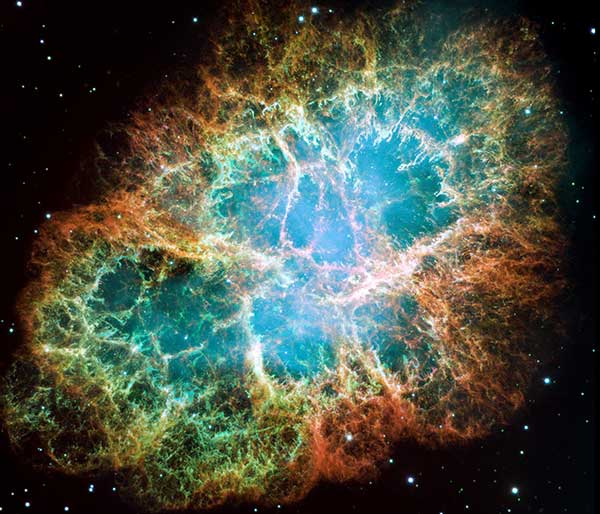
\includegraphics[width=6cm]{files/crab_optical_full.jpg}
	\end{center}
\end{frame}
%
\subsection{Ultravioletti}
\begin{frame}[ultravioletti]
	\frametitle{Gli ultravioletti}
	\begin{center}
		{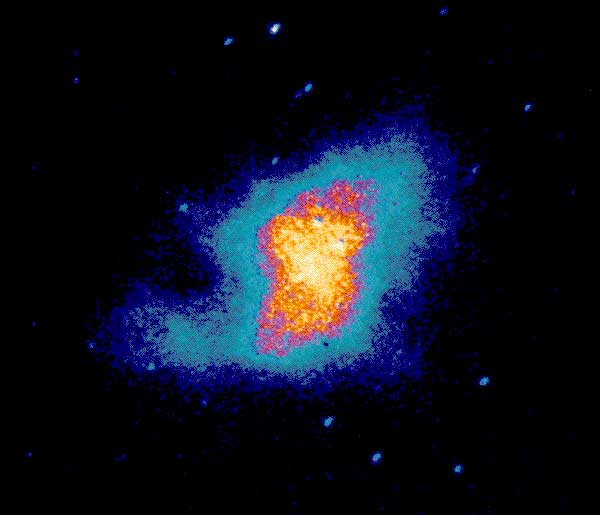
\includegraphics[width=6cm]{files/crab_uv_full.jpg}}
	\end{center}
\end{frame}
%
\subsection{Raggi-X}
\begin{frame}[raggix]
	\frametitle{Raggi-X}
	\begin{center}
		{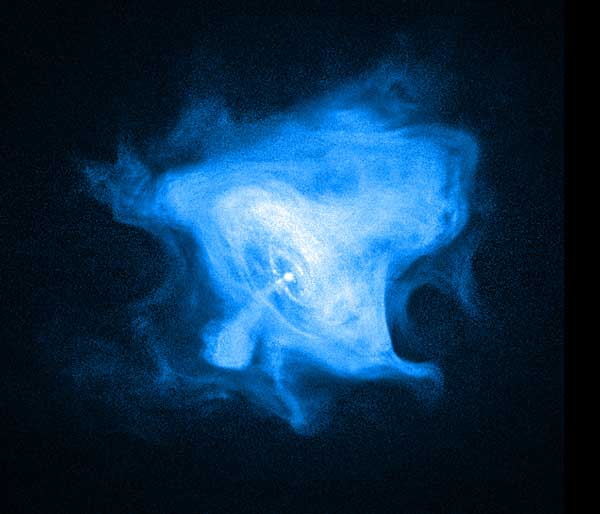
\includegraphics[width=6cm]{files/crab_xray_full.jpg}}
	\end{center}
\end{frame}
%
\section{L'universo ottico}
\begin{frame}[ottico01]
	\frametitle{I concetti fondamentali}
	\begin{itemize}
		\item La sfera celeste
		\item L'eclittica
		\item Costellazioni e Via Lattea
		\item Coordinate geografiche e celesti
		\item Declinazione
		\item Moti reali e moti apparenti
		\item Alba e tramonto degli astri
	\end{itemize}
	\href{http://edu.iasfbo.inaf.it/moodle/course/view.php?id=3}{\textcolor{inaf}{Moodle delle Olimpiadi di Astronomia}}
\end{frame}
%
\begin{frame}[ottico02]
	\frametitle{Le grandezze da misurare}
	\begin{itemize}
		\item Luminosit�
		\item Legge di Pogson
		\item Magnitudine
	\end{itemize}
\end{frame}
%
\subsection{La sfera celeste}
%
\begin{frame}[sfera_celeste01]
	\frametitle{La sfera celeste}
	\begin{block}{}
		Sfera di raggio arbitrario sulla cui superficie sono proiettati tutti gli astri.\\
	\end{block}
\end{frame}
%
\begin{frame}[sfera_celeste02]
	\frametitle{Riferimenti}
	\begin{itemize}
		\item<1-> zenit
		\item<2-> nadir
		\item<3-> meridiano celeste
		\item<4-> punto di mezzocielo
		\item<5-> orizzonte astronomico
	\end{itemize}
\end{frame}
%
\begin{frame}[sfera_celeste03]
	\frametitle{Coordinate celesti e declinazione}
	\scriptsize
	\begin{block}{Sistema equatoriale}
		Prende come riferimento l'equatore celeste, ovvero l'intersezione tra l'equatore terrestre e la sfera celeste.
	\end{block}
	\onslide<2->
	\begin{itemize}
		\item<2-> ascensione retta (longitudine)
		\item<3-> declinazione (latitudine)
	\end{itemize}
\end{frame}
%
\subsection{La Via Lattea}
%
\begin{frame}[via_lattea]
	\frametitle{La sfera celeste}
	\begin{center}
		{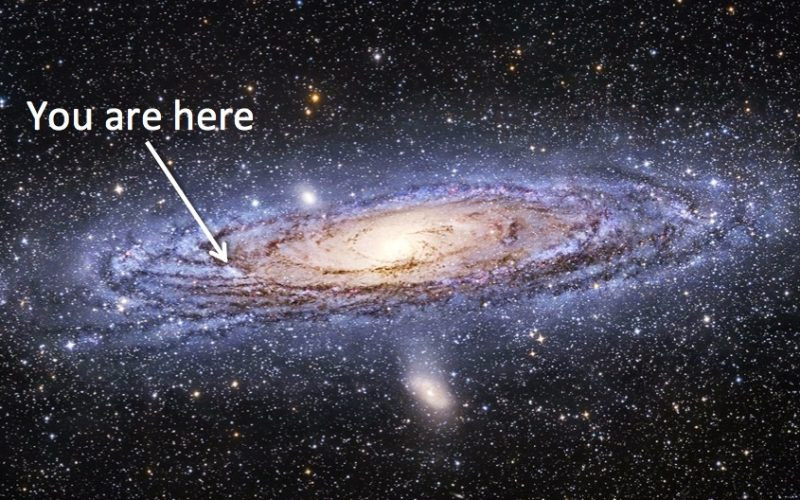
\includegraphics[width=6cm]{files/milky_way.jpg}}
	\end{center}
	Esempio: EduINAF: \href{http://edu.inaf.it/index.php/attivita_didattica/costruzione-del-sistema-solare-in-scala/}{\textcolor{inaf}{Costruzione del Sistema Solare in scala}}\\
	Esempio: astroEDU \href{http://astroedu.iau.org/it/activities/1512/un-modello-del-sistema-solare-sulla-mappa-della-citta/}{\textcolor{inaf}{Un modello del Sistema Solare sulla mappa della citt�}}\\
	Video: \href{https://www.youtube.com/watch?v=0fKBhvDjuy0}{\textcolor{inaf}{Powers of ten}}
\end{frame}
%
\subsection{Cosa si misura}
%
\begin{frame}[lumi01]
	\frametitle{Luminosit�}
	\begin{block}{}
		La quantit� di energia elettromagnetica emessa da una stella per unit� di tempo. Si misura pertanto in watt, in erg/secondo oppure in luminosit� solare.
		\[F=\frac{L}{A}\]
		dove $F$ � la densit� del flusso, $A$ la superficie
	\end{block}
\end{frame}
%
\begin{frame}[lumi02]
	\frametitle{Luminosit�: Legge di Pogson}
	\scriptsize
	\begin{block}{Luminosit� intrinseca}
		\[L = \frac{L_0}{4 \pi d^2}\]
		dove $L_0$ luminosit� intrinseca, $L$ luminosit� osservata, $d$ distanza dalla stella
	\end{block}
	\onslide<2->
	\begin{block}{Magnitudine apparente}
		\[m = -2.5 \log_{10}{F} + c\]
		dove $F$ flusso osservato, $c$ costante
	\end{block}
	\onslide<3->
	\begin{block}{Flusso}
		\[F = \frac{L}{4 \pi d^2}\]
	\end{block}
\end{frame}
%
\begin{frame}[lumi03]
	\frametitle{Luminosit�}
	\scriptsize
	\begin{block}{Magnitudine assoluta}
		\[M = m - 5((\log_{10}{d})-1)\]
		dove $L_0$ luminosit� intrinseca, $L$ luminosit� osservata, $d$ distanza dalla stella
	\end{block}
	\onslide<2->
	\begin{block}{Distanza}
		\[d = 10^{\frac{M-m-5}{5}}\]
	\end{block}
	\onslide<3->
	\begin{block}{Legge di Stefan-Boltzmann}
		\[L = 4 \pi R^2 \alpha T^4\]
	\end{block}
\end{frame}
%
\section{Bibliografia}
%
\begin{frame}[bibliografia]
	\frametitle{Bibliografia}
	\begin{itemize}
		\item \href{https://it.wikibooks.org/wiki/Fisica_classica/Spettro_delle_onde_elettromagnetiche}{\textcolor{inaf}{Wikibooks: Fisica classica/Spettro delle onde elettromagnetiche}}
		\item \href{https://it.wikipedia.org/wiki/Spettro_elettromagnetico}{\textcolor{inaf}{Wikipedia: Spettro elettromagnetico}}
		\item \href{https://www.matematicamente.it/appunti/fisica-per-le-superiori/elettromagnetismo-fisica-per-le-superiori/lo-spettro-elettromagnetico/}{\textcolor{inaf}{Lo spettro elettromagnetico di Francesca Ricci}}
		\item \href{https://www.pbslearningmedia.org/resource/phy03.sci.ess.eiu.chandra/astronomical-images-in-different-wavelengths/}{\textcolor{inaf}{Astronomical Images in Different Wavelengths}}
	\end{itemize}
\end{frame}
\end{document}
